\chapter{Kanban Setup \\
\small{\textit{-- Nicole Valdiviezo}}
\index{Kanban Setup} 
\index{Chapter!Kanban Setup}
\label{Chapter::Kanban Setup}}

To manage the workflow of the DevOpsConfiguration project, I set up a Kanban board using Atlassian JIRA. The following steps outline the setup process:

\begin{enumerate}
    \item  Logged into the Atlassian JIRA cloud platform with my account.
    \item Created a new project and selected the \textbf{Kanban software development} template.
    \item Named the project \textbf{SSW}.
    \item Defined the basic Kanban workflow with three columns: \textbf{To Do}, \textbf{In Progress}, and \textbf{Done}.
    \item Added automation rules so that when an issue is marked as resolved, it automatically moves to the \textbf{Done} column.
    \item Populated the board with initial tasks such as ``Complete first assignment,'' ``Setup Kanban Board,'' and ``Compile project into Overleaf.''
\end{enumerate}

This Kanban setup provides visibility into task progress, supports iterative development, and aligns with agile DevOps practices.


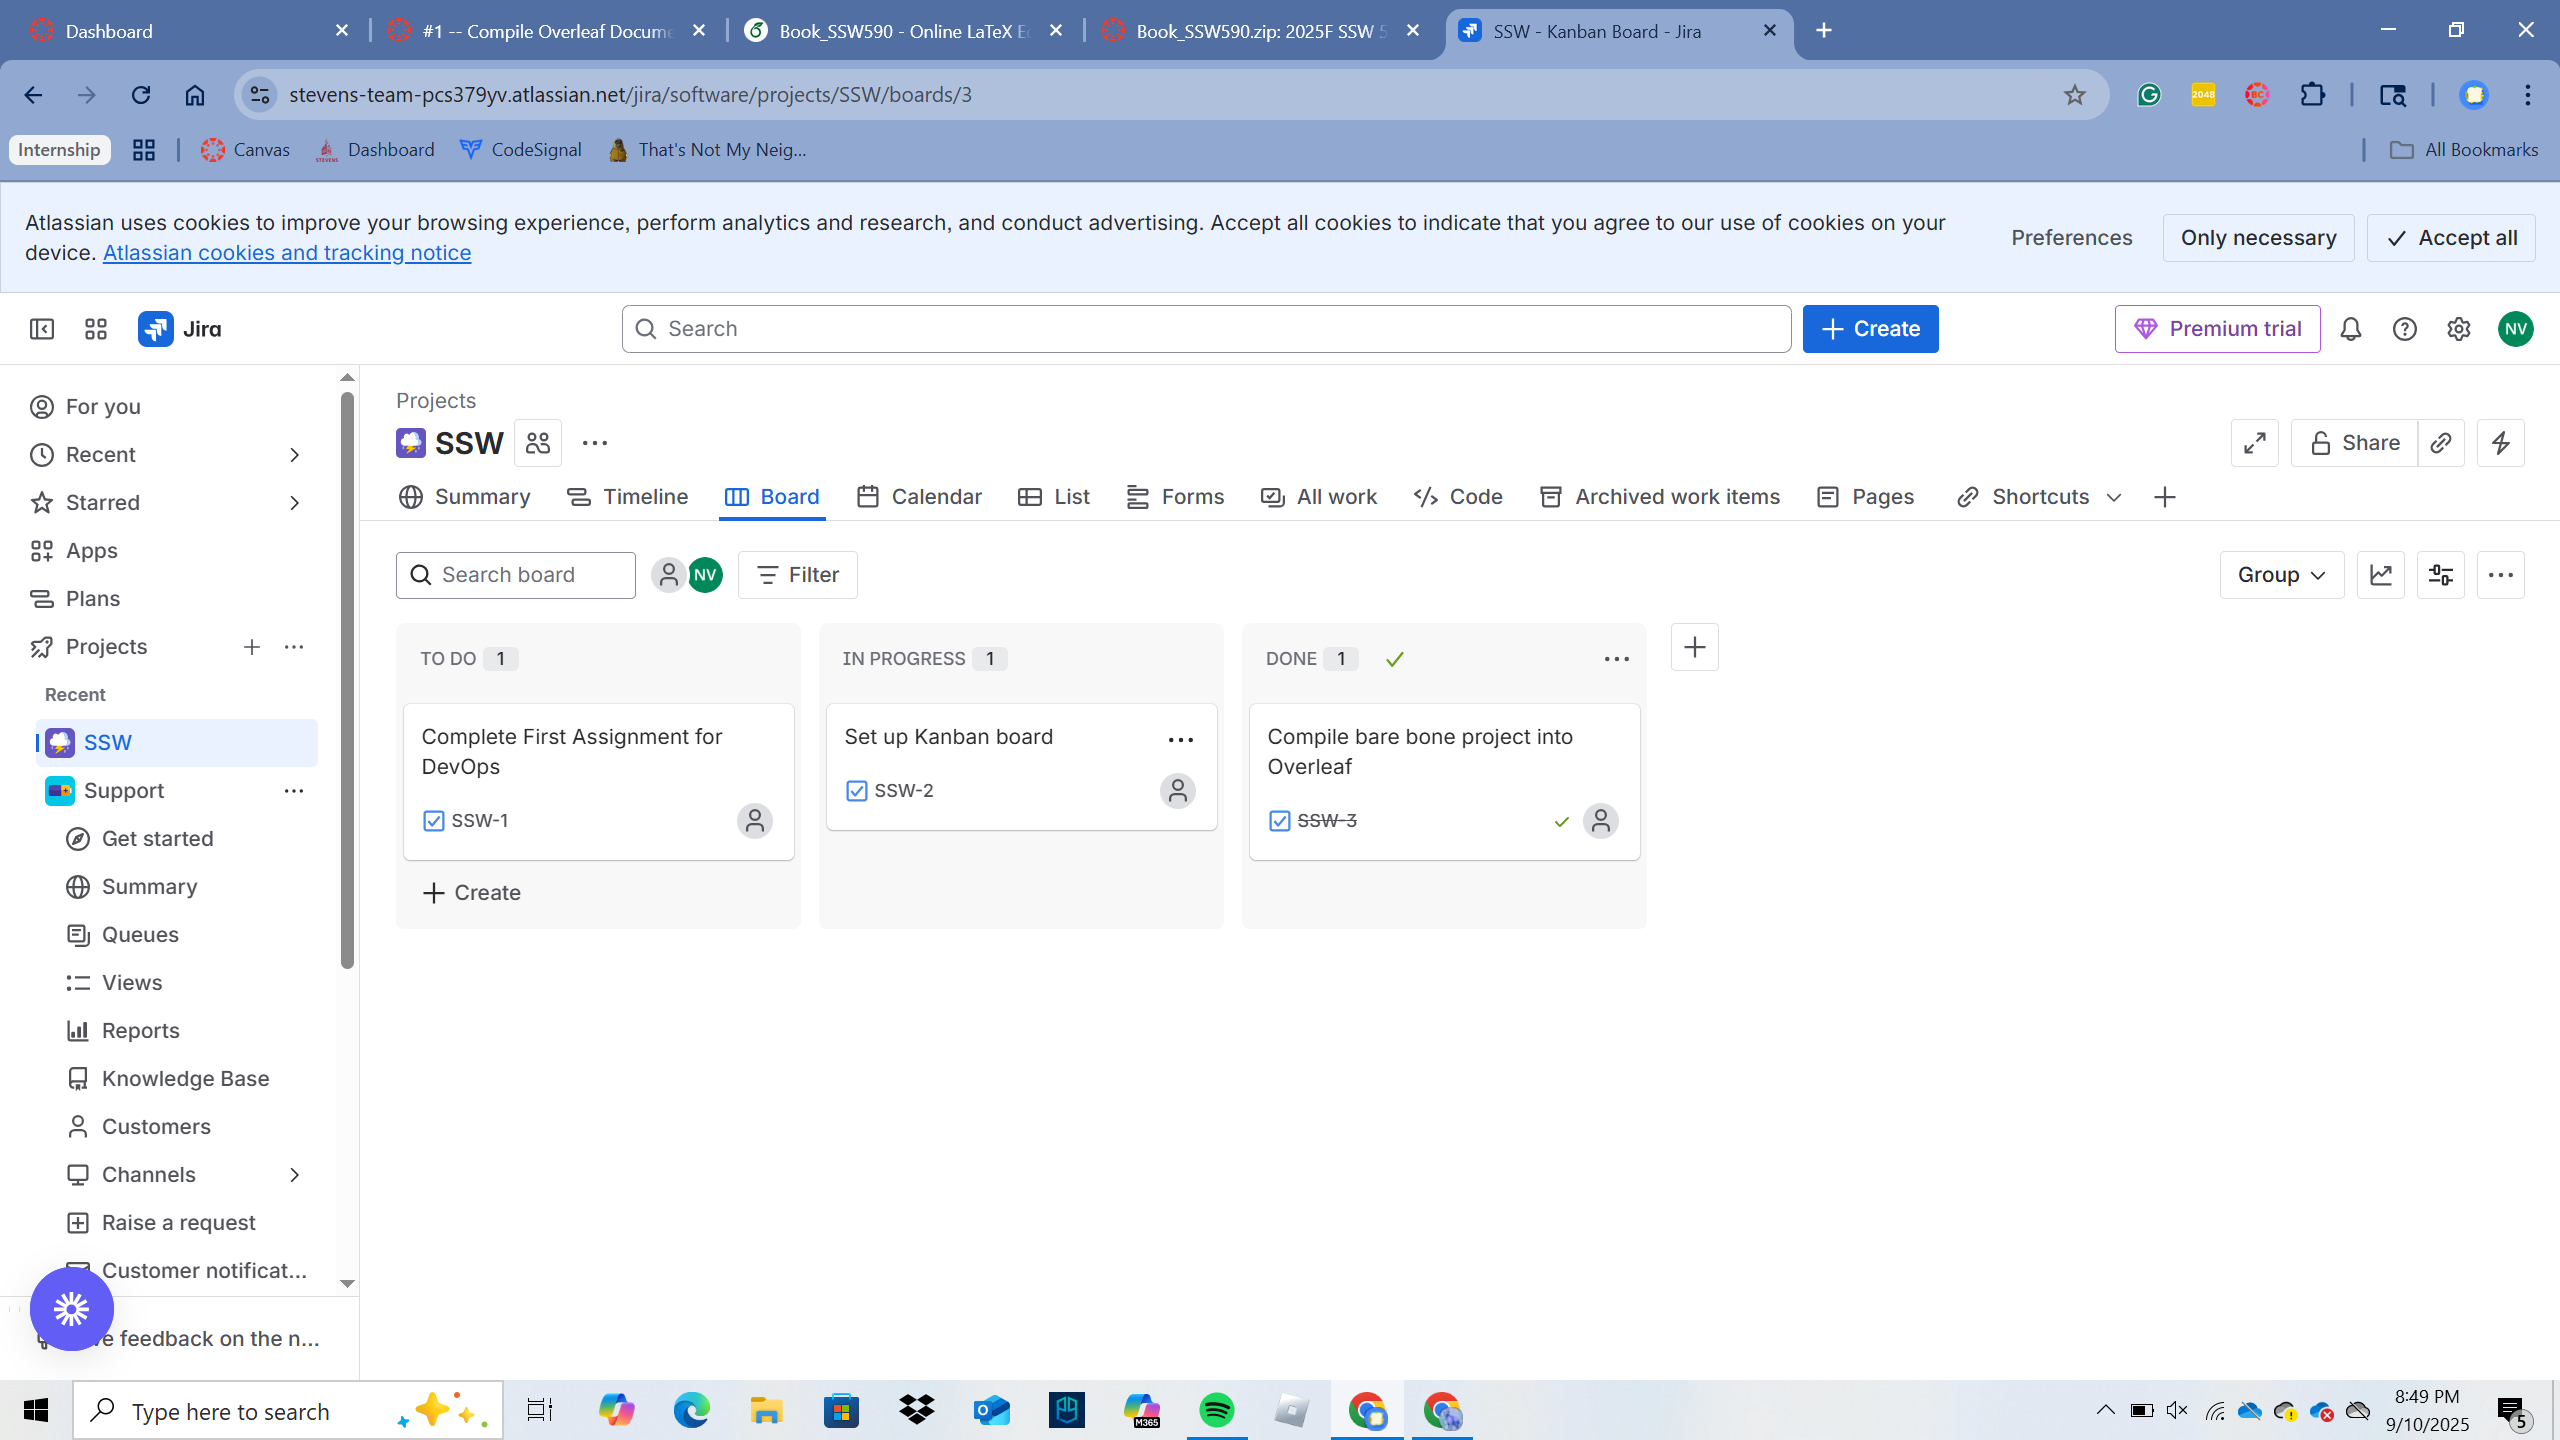
\includegraphics[scale=0.1]{eps/Screenshots/Screenshot (255).png}
